\section{Data and design}
\label{sec:design}
We draw on two datasets, one publicly available and one created by us, to
uncover Tor relays that behave and look similarly.  Our detection methods are
implemented in a tool, sybilhunter, which takes as input archived Tor network
data and then attempts to expose Sybil groups, as illustrated in
Figure~\ref{fig:system}.  While developing sybilhunter, we faced many design
decisions that we tackled by drawing on the experience we gained by manually
analyzing numerous Sybil relay groups.  We iteratively improved sybilhunter when
we experienced operational shortcomings and augmented our design with ideas from
related work, e.g., Cao et al. observed that Sybil groups share properties and
frequently change at the same time~\cite{Cao2014a}.

\begin{figure}[t]
	\centering
	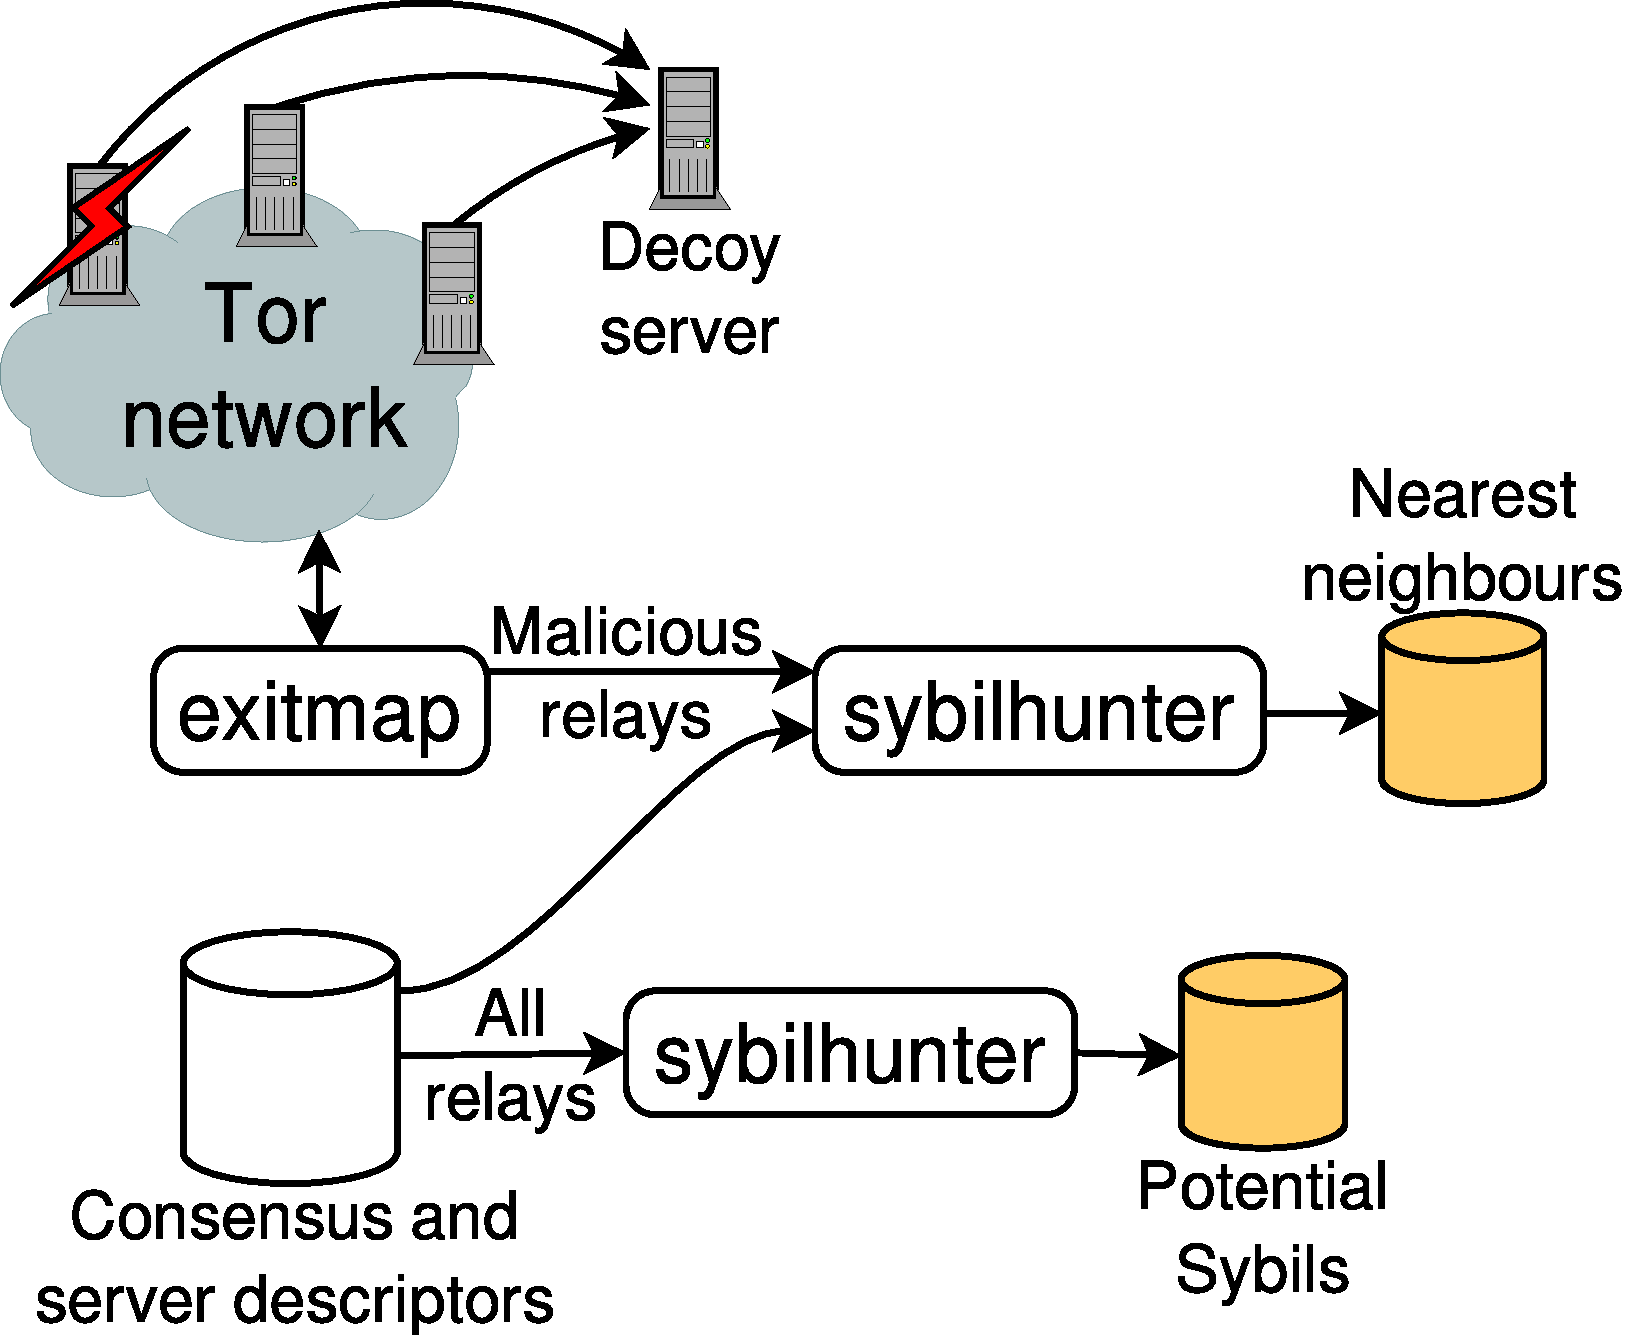
\includegraphics[width=0.4\textwidth]{diagrams/system_architecture.pdf}
	\caption{Our system architecture.  Two datasets serve as input to
		sybilhunter: archived consensuses and server descriptors, and malicious
		relays that we gather by running exitmap~\cite{Winter2014a}.
		Sybilhunter then attempts to extract Sybil groups from the given data.}
	\label{fig:system}
\end{figure}

Generally speaking, sybilhunter seeks to expose relays that are similar in their
\emph{behavior} and \emph{appearance}; we designed it to 1) run over historical
network data, dating back to 2007; 2) run over online data, to detect new Sybils
as they join the network; and 3) find relays that might be associated with
previously discovered, malicious relays.

\subsection{Datasets}
\label{sec:datasets}
Figure~\ref{fig:system} shows how we use our two datasets.  Archived consensuses
and router descriptors (in short: descriptors) allow us to 1) restore past
states of the Tor network, which we mine for Sybil groups, and to 2) find
``partners in crime'' of malicious exit relays that we discovered by running the
exitmap scanner.

\subsubsection{Consensuses and router descriptors}
The consensus and router descriptor dataset is publicly available on
CollecTor~\cite{collector}, a service that is run by The Tor Project to archive
network data such as consensuses, router descriptors, and network status votes.
Some of the archived data dates back to as early as 2004, allowing us to restore
arbitrary Tor network states in the last ten years.  Not all of CollecTor's
archived data, however, is relevant to our hunt for Sybils, which is why we only
analyse the following two:

\begin{figure}[t]
	\centering
	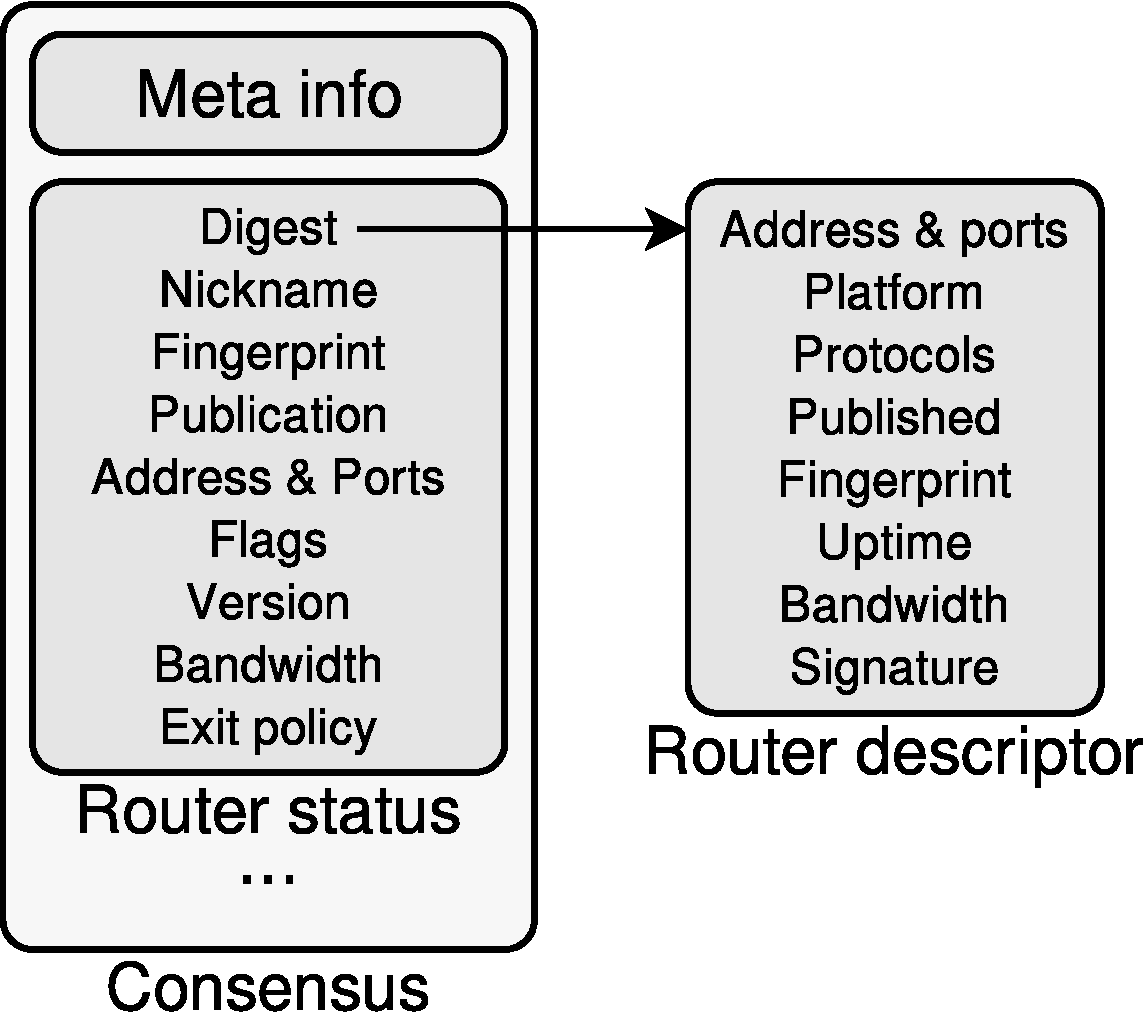
\includegraphics[width=0.3\textwidth]{diagrams/data_sets.pdf}
	\caption{Our dataset contains consensuses (produced by directory
		authorities) and router descriptors (produced by relays).  Every hour,
		a new consensus is generated, and relays upload their router descriptor
		at least every 18 hours.}
	\label{fig:datasets}
\end{figure}

\begin{description}
	\item[Descriptors] Tor relays and bridges periodically upload router
		descriptors, which capture their configuration, to directory
		authorities.  Relays upload their descriptors no later than every 18
		hours, or sooner, depending on certain conditions.  Note that some
		information in router descriptors is not verified by directory
		authorities.  As a result, relays are able to spoof information such as
		their operating system, Tor version, and uptime.

	\item[Consensuses] Every hour, directory authorities vote on the state of
		the network, producing the consensus, which is a list of all running Tor
		relays.  Every relay status in the consensus contains a digest that
		points to the relay's descriptor.
\end{description}

Figure~\ref{fig:datasets} illustrates the relationship between our data.
Primarily, we are interested in the hourly consensus files.  A consensus file
consists of \emph{router statuses} that contain basic information about Tor
relays such as its bandwidth, flags, and exit policy.  As of Nov 2015,
consensuses contain almost 7,000 router statuses, i.e., every hour, 7,000 router
statuses are published, and archived by CollecTor.  Every router status contains
a digest that is used to locate its corresponding \emph{router descriptor}.
Again, router descriptors are published as they were received by Tor relays
while consensus files are voted on, and published, by directory authorities.
Some fields in a router status are also subject to verification.  For example,
the Tor network operates bandwidth scanners that verify if a relay is able to
sustain the bandwidth it claims to handle in its router descriptor.

Table~\ref{tab:collector-dataset} gives an overview of the size of our dataset.
We found it challenging to process these millions of files, adding up to almost
100 GiB of uncompressed data.  In our first processing attempt, we used the
Python parsing library Stem~\cite{stem}, which is maintained by The Tor Project.
The size of data and number of files turned out to be difficult to handle for
Stem because of Python's interpreted and dynamic nature.  To process our dataset
more efficiently, we implemented a custom parser in the Go programming
language~\cite{zoossh}.  Our parser consists of approximately 1,300 lines of
code (and 800 additional lines for tests) and supports both strict and lazy
parsing.  According to our benchmarks, our parser can process approximately 27
consensuses per second, as measured on an Intel Core i7 2.9 GHz CPU, a
consumer-grade CPU.  We placed our datasets on a solid state drive to eliminate
the I/O bottleneck.  Stem, for comparison, averages at around 1.8 consensuses
per second.  Note, however, that Stem processes more fields than our parser,
which makes it difficult to have a fair comparison.

\begin{table}[t]
\centering
\begin{tabular}{l c c c}
\textbf{Dataset} & \textbf{\# of files} & \textbf{Size} & \textbf{Time span} \\
\hline
% find . -type f | wc -l
% du -b consensuses/
Consensuses & 69,877 & 47 GiB & 10/2007 -- 10/2015 \\
Descriptors & 32,376,097 & 47 GiB & 12/2005 -- 10/2015 \\
\end{tabular}
\caption{An overview of our first dataset, consensuses and server descriptors
since 2007 and 2005, respectively.}
\label{tab:collector-dataset}
\end{table}

\subsubsection{Malicious relays}
We used a second, complementary dataset, shown in
Table~\ref{tab:exitmap-dataset}, that consists of malicious exit relays we
gathered by running Winter's exitmap tool~\cite[\S 3.1]{Winter2014a} over 15
months.  Exitmap is a Python-based scanning framework for Tor exit relays.
Exitmap modules perform a network task that can then be run over all exit
relays.  One use case is HTTPS MitM detection: A module can fetch the X.509
certificate of a web server over all exit relays and then compare the
fingerprint with the expected, valid fingerprint.  In addition to the original
modules that the exitmap authors shared with us, we implemented modules to
detect HTML tampering and TLS downgrading, by connecting to servers under our
control and raising an alert if the returned HTML or received TLS server hello
were modified.  Our modules ran from August 2014 to November 2015 and discovered
205 malicious exit relays, which we all reported to The Tor Project.

\begin{table}[t]
\centering
\begin{tabular}{l c p{4cm}}
\textbf{Discovery} & \textbf{\# of relays} & \textbf{Attack description} \\
\hline
% Message-ID: <20151117150055.GA25187@nymity.ch>
2015-11-17 & 8$\dagger$ & Downgrade TLS and replace onion domains. \\
% Message-ID: <20151116164403.GL10892@nymity.ch>
2015-11-16 & 1 & SSLStrip attack. \\
% Message-ID: <20150908174557.GG8901@nymity.ch>
2015-09-08 & 1 & Injects iframe into relayed HTML. \\
% Message-ID: <20150804202838.GA4774@nymity.ch>
2015-08-04 & 4$\dagger$ & Onion service impersonation by rewriting onion domains. \\
% Message-ID: <20150630022923.GA2340@nymity.ch>
2015-06-29 & 55$\dagger$ & Onion service impersonation by rewriting onion domains. \\
% Message-ID: <20150423004031.GA11395@nymity.ch>
2015-04-22 & 70$\dagger$ & Onion service impersonation by rewriting onion domains. \\
% Message-ID: <20150311125831.GD23215@nymity.ch>
2015-03-11 & 1 & Injected iframe into relayed HTML. \\
% Message-ID: <20150311131506.GE23215@nymity.ch>
2015-03-11 & 18$\ddagger$ & Bitcoin site MitM. \\
2015-02-11 & 17$\ddagger$ & Bitcoin site MitM. \\
% Message-ID: <20150210154109.GD10777@nymity.ch>
2015-02-10 & 1 & Injects advertisement into HTML. \\
2015-01-10 & 1 & Incorrect DNS resolution. \\
% Message-ID: <20150109195428.GA29115@nymity.ch>
2015-01-09 & 23$\ddagger$ & Bitcoin site MitM. \\
% Message-ID: <20141025182433.GA23244@nymity.ch>
2014-10-25 & 1 & Running sslstrip. \\
% Message-ID: <20141021133016.GA11247@nymity.ch>
2014-10-21 & 1 & Running sslstrip. \\
% Message-ID: <20141021133016.GA11247@nymity.ch>
2014-10-21 & 1 & Injecting JavaScript into HTML. \\
% Message-ID: <20140920132357.GC8751@nymity.ch>
2014-09-20 & 1 & Routes traffic back into the Tor network. \\
% Message-ID: <20140831153809.GA1799@nymity.ch>
2014-08-31 & 1 & Injecting JavaScript into HTML. \\
% Message-ID: <20140811014615.GB23748@nymity.ch>
2014-08-10 & 1 & Injecting JavaScript into HTML. \\
\end{tabular}
\caption{An overview of our second dataset, 205 bad exit relays we discovered
	between Aug 2014 and Nov 2015.  We believe that all single relays in
	the dataset were isolated incidents while multiple relays constituted Sybil
	clusters.  Sybil groups marked with a $\dagger$ or a $\ddagger$ were run by
	the same attacker.}
\label{tab:exitmap-dataset}
\end{table}

We add malicious exit relays to our dataset because these relays frequently
\emph{surface in groups}, i.e., an attacker runs the same attack on several,
physically distinct exit relays~\cite{Winter2014a}.  Winter et al.'s
work~\cite[\S 5.2]{Winter2014a} further showed that attackers make an effort to
stay under the radar, which is why we cannot only rely on active probing to find
and block such relays.  We also seek to find the \emph{nearest neighbors} of
each newly discovered malicious relay, which we discuss in
Section~\ref{sec:nearest-neighbor}.

\subsection{Threat model}
\label{sec:threat_model}
When we apply sybilhunter on newly incoming data, adversaries can manipulate
their Sybil configuration to evade our system, and the powerful nature of Sybil
attacks~\cite{Douceur2002a} limits our defenses.  This is reflected in our
adversarial assumptions.  We assume that our adversaries \emph{do}:
\begin{itemize}
	\item Run more than one Tor relay.

	\item Have redundancy in their behavior or appearance, e.g., similar
		configuration.
\end{itemize}

Our adversaries further \emph{can}:
\begin{itemize}
	\item Add Tor relays all at once or slowly over time.

	\item Run active or passive attacks.

	\item Make a limited effort to stay under the radar by diversifying
		different parts of their relay configuration.
\end{itemize}

% TODO (23 Nov 2015, 11:01am): Maybe elaborate that our methods fail if Sybils
% exhibit no redundancy.

\subsection{Analysis techniques}
\label{sec:techniques}
We now turn to presenting techniques that can expose Sybils in our datasets
(\S~\ref{sec:datasets}) under our given threat model
(\S~\ref{sec:threat_model}).

\subsubsection{Network churn time series}
\label{sec:churn-time-series}
The churn rate of a distributed system is the rate of joining and leaving
network participants---relays in the Tor network.  An unexpectedly high churn
rate between two subsequent consensuses can reveal Sybils because Sybil
operators frequently start and stop their Sybils at the same time for convenient
administration.

The Tor Project is maintaining a Python script~\cite{doctor} that determines the
number of relay fingerprints in new consensuses that have never been seen
before.  If that number exceeds the static threshold 49, an email alert is sent.
We reimplemented the script in sybilhunter and ran it over all archived
consensus documents, dating back to 2007.  The script raised 47 alerts in nine
years, all of which seemed true positives, i.e., they should be of interest to
directory authority operators.  The script did not raise false positives because
the median number of new fingerprints in a consensus is only six---significantly
below the conservative threshold of 49.  The script's conservative threshold
probably causes false negatives, but we cannot determine the false negative rate
because we lack ground truth.  In addition, The Tor Project's script can be
defeated by a ``trickling'' attack in which Sybils are slowly added over time.
We now extend The Tor Project's approach to make it more robust against these
shortcomings.

We found that churn anomalies worthy of our attention range from \emph{flat
hills} (see Figure~\ref{fig:flat-hill}) to \emph{sudden spikes} (see
Figure~\ref{fig:sudden-spike}).  The former can be a sign of an event that
affected a large number of relays in the network\footnote{This happened shortly
after the heartbleed vulnerability when The Tor Project asked relay operators
to generate new keys.  Naturally, relay operators did not do this at the same
hour, but gradually over approximately two days.} while the latter can happen if
an attacker adds relays over time, or an external event causes an influx of
relays.

\begin{figure}[t]
	\centering
	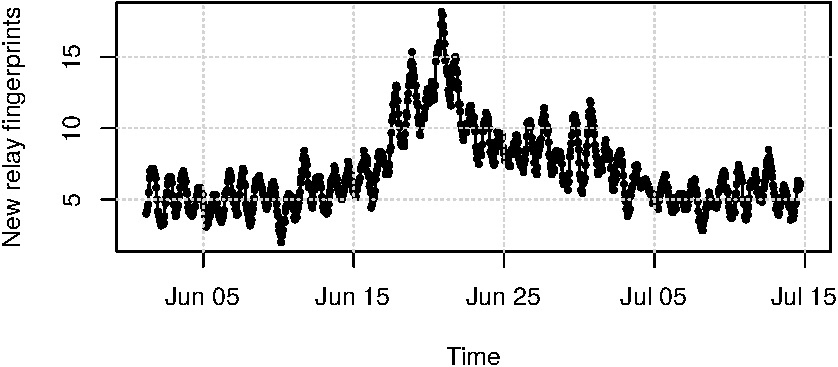
\includegraphics[width=\linewidth]{diagrams/flat-hill.pdf}
	\caption{A flat hill in 2009.  The time series was smoothed using a moving
	average with a window size of 12 hours.}
	\label{fig:flat-hill}
\end{figure}

\begin{figure}[t]
	\centering
	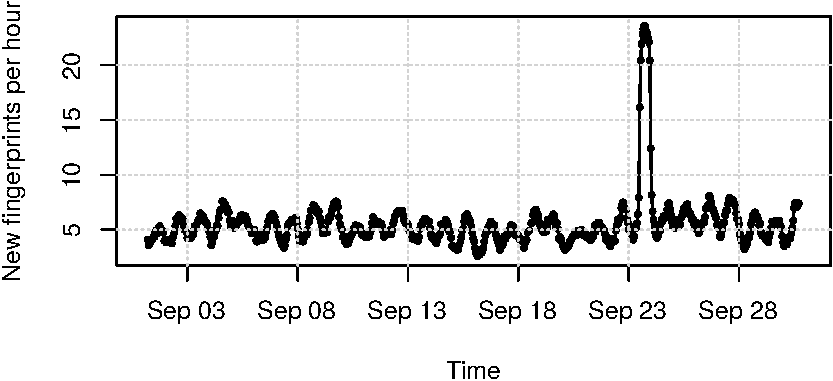
\includegraphics[width=\linewidth]{diagrams/sudden-spike.pdf}
	\caption{A sudden spike in 2010.  The time series was smoothed using a
	moving average with a window size of 12 hours.}
	\label{fig:sudden-spike}
\end{figure}

To quantify the churn rate $\sigma$ between two subsequent consensus documents,
we adapt Godfrey et al.~\cite{Godfrey2006a} formula which yields a single churn
value that captures both new and gone systems.  That means that an unusually low
number of gone systems could cancel out an unusually high number of new
systems---an undesired property for a system that should highlight abnormal
changes.  To address this issue, we split the formula in two parts and create a
time series for new relays ($\sigma_{n}$) as well as for gone relays
($\sigma_{g}$).  $C_{t}$ is the network consensus at time $t$, and $\setminus$
denotes the complement between two consensuses, i.e., the number of relays that
is in one consensus, but not the other.  We now define $\sigma_{n}$ and
$\sigma_{g}$ as:

\begin{equation}
\sigma_{n} = \frac{\lvert C_{t} \setminus C_{t-1} \rvert}
{\textrm{max}\{\lvert C_{t-1} \rvert, \lvert C_{t} \rvert \}}
\end{equation}

\begin{equation}
\sigma_{g} = \frac{\lvert C_{t-1} \setminus C_{t} \rvert}
{\textrm{max}\{\lvert C_{t-1} \rvert, \lvert C_{t} \rvert \}}
\end{equation}

$\sigma_{n}$ and $\sigma_{g}$ are bounded to the interval $[0, 1]$.  A churn
value of 0 indicates no change between two subsequent consensuses whereas a
churn value of 1 indicates a complete network turnover.  Determining
$\sigma_{n,g}$ for the sequence $C_{t}, C_{t-1}$, $C_{t-2}$, \ldots, yields a
time series of churn values that can readily be inspected for abnormal spikes as
the one in Figure~\ref{fig:sudden-spike}.  To detect changes in the underlying
trend, we can smooth $\sigma_{n,g}$ using a simple moving average $\lambda$,
defined as:

\begin{equation}
\lambda = \frac{1}{w} \cdot \sum_{i=0}^{w} \sigma_{i}
\end{equation}

As we increase the window size $w$, we are able to detect more subtle changes in
the underlying trend.  In an operational setting, we believe that this parameter
should be kept secret because otherwise it would help attackers to stay under
the radar.  Refer to Section~\ref{sec:secrecy} for a comprehensive discussion on
this transparency and secrecy tradeoff.  If $\lambda$ or $\sigma_{n,g}$ exceed a
manually defined threshold, an alert is raised.

% \mynote{We could plot the number of alerts we would get for a sequence of
% thresholds.}

\subsubsection{Uptime matrix}
\label{sec:uptime-matrix}
An unexpectedly high churn rate can indicate a significant network event, but it
does not reveal \emph{which relays} are responsible for this event.  It captures
the state of the network, but not of individual relays.  To bridge this gap, we
now propose an analysis technique for the uptime of single relays.

We now take a step back to understand why relay uptimes are relevant.  For
convenience, attackers are likely to administer their Sybil relays in parallel,
i.e., update, configure, and reboot them simultaneously.  This is reflected in
the hourly uptime of Tor relays.  If an attacker decides to install an operating
system upgrade on all of her Sybils, we might observe a cluster of relays going
offline and back online all at the same time.  To isolate such events, we are
comparing \emph{uptime patterns} of Tor relays.  Relays featuring a similar
uptime pattern are more likely to be under common control than relays with a
distinct uptime pattern.

We represent uptime patterns as a binary sequences.  Every hour, when a new
consensus is published, we append a new data point to the sequence for each Tor
relay.  It is tempting to quantify the similarity between two relays with the
Hamming distance, defined as the amount of positions
at which two strings of equal length differ.  This, however, does not perfectly
capture our intuition as we show in Figure~\ref{fig:uptime-pattern}.  Relay $B$
and $C$ have the same Hamming distance to relay $A$: two.  Intuitively, however,
we consider relay $B$ to be more similar to relay $A$ than is $C$ because it
does not exhibit the uptime sequence at hour seven and eight.  We account for
this by increasing a \emph{deviation amplifier} as two uptime sequences
continue to diverge (see Algorithm~\ref{alg:uptime}).  As long as two sequences
keep deviating, our deviation amplifier is increased by 0.1 until it reaches 1.
As soon as two sequences converge again, the deviation error is reset to 0.
Finally, we divide the distance by the sequence length to normalize it to the
interval $[0, 1]$.  According to this algorithm, relay $A$ and $B$ in
Figure~\ref{fig:uptime-pattern} have a similarity of 0.1 + 0.1 while $A$ and $C$
have a similarity of 0.1 + 0.2.

% \mynote{Uptime sequences in Algorithm~\ref{alg:uptime} should probably deviate
% exponentially rather than linearly.}

\begin{figure}[t]
\centering
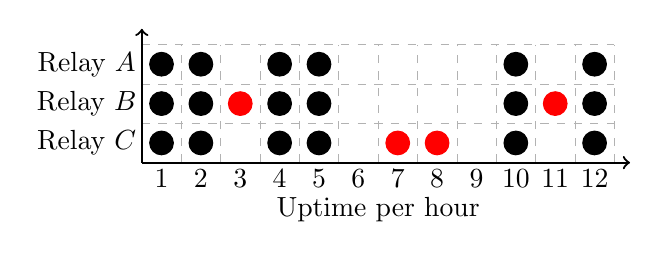
\begin{tikzpicture}
\draw[help lines, color=gray!60, dashed, step=0.5] (0,0) grid (6,1.5);
\draw[->,thick] (0,0)--(6.2,0);
\draw[->,thick] (0,0)--(0,1.7);

% Y labels.
\node at (-0.7,1.25) {Relay $A$};
\node at (-0.7,0.75) {Relay $B$};
\node at (-0.7,0.25) {Relay $C$};

% X labels.
\node at (0.25, -0.2) {1};
\node at (0.75, -0.2) {2};
\node at (1.25, -0.2) {3};
\node at (1.75, -0.2) {4};
\node at (2.25, -0.2) {5};
\node at (2.75, -0.2) {6};
\node at (3.25, -0.2) {7};
\node at (3.75, -0.2) {8};
\node at (4.25, -0.2) {9};
\node at (4.75, -0.2) {10};
\node at (5.25, -0.2) {11};
\node at (5.75, -0.2) {12};

\node at (3, -0.6) {Uptime per hour};

% Relay A.
\filldraw[black] (0.25,1.25) circle (0.15);
\filldraw[black] (0.75,1.25) circle (0.15);

\filldraw[black] (1.75,1.25) circle (0.15);
\filldraw[black] (2.25,1.25) circle (0.15);

\filldraw[black] (4.75,1.25) circle (0.15);

\filldraw[black] (5.75,1.25) circle (0.15);

% Relay B.
\filldraw[black] (0.25,0.75) circle (0.15);
\filldraw[black] (0.75,0.75) circle (0.15);
\filldraw[red]   (1.25,0.75) circle (0.15);
\filldraw[black] (1.75,0.75) circle (0.15);
\filldraw[black] (2.25,0.75) circle (0.15);

\filldraw[black] (4.75,0.75) circle (0.15);
\filldraw[red]   (5.25,0.75) circle (0.15);
\filldraw[black] (5.75,0.75) circle (0.15);

% Relay C.
\filldraw[black] (0.25,0.25) circle (0.15);
\filldraw[black] (0.75,0.25) circle (0.15);

\filldraw[black] (1.75,0.25) circle (0.15);
\filldraw[black] (2.25,0.25) circle (0.15);

\filldraw[red]   (3.25,0.25) circle (0.15);
\filldraw[red]   (3.75,0.25) circle (0.15);

\filldraw[black] (4.75,0.25) circle (0.15);

\filldraw[black] (5.75,0.25) circle (0.15);
\end{tikzpicture}

\caption{Uptime pattern of three relays.  Intuitively, relay $B$ is more
similar to relay $A$ than is relay $C$, but the Hamming distance is two for
both patterns.}
\label{fig:uptime-pattern}
\end{figure}

\begin{algorithm}[t]
\SetKwData{Dist}{dist}
\SetKwData{Amp}{amp}
\SetKwData{Hours}{hours}
\SetKwData{Result}{result}
\SetKwInOut{Input}{input}
\SetKwInOut{Output}{output}

\Input{$A$ and $B$, two uptime patterns}
\Output{$\Result$}
\BlankLine
$\Dist \leftarrow 0$\;
$\Amp \leftarrow 0$\;
\ForEach{$t \in \Hours$}{
    \eIf{$A_{t} \ne B_{t}$}{
        \If{$\Amp < 1$}{
            $\Amp \leftarrow \Amp + 0.1$\;
        }
    $\Dist \leftarrow \Dist + \Amp$\;
    }{
        $\Amp \leftarrow 0$\;
    }
}
$\Result \leftarrow \Dist / \lvert \Hours \rvert$\;
\caption{Our algorithm to quantify the similarity between the uptime pattern
of two relays $A$ and $B$.}
\label{alg:uptime}
\end{algorithm}

We employ Algorithm~\ref{alg:uptime} in a visualization that sybilhunter can
generate for a given set of consensuses.  The visualization is a bitmap whose
rows denote hours, and whose columns denote relays.  Every pixel in the image
represents the uptime status of a given relay.  If the pixel is black, the relay
is online, and if it is white, it is offline.  Note that this type of
visualization was first proposed by Ensafi and subsequently implemented by
Fifield~\cite{Fifield2014a}.  Similar to Fifield, we sort columns to group
similar uptime patterns together.  Our first sorting criteria is the amount of
hours a relay was online, and our second criteria is the median value of the
online sequence.  Figure~\ref{fig:uptime-matrix} gives an example, illustrating
the uptime patterns for relays in September 2011.  As columns increase, so does
the uptime of relays, until they are almost always online.  Sybils with similar
uptimes manifest as solid ``blacks'' in this type of visualization.  Refer to
Section~\ref{sec:fingerprint-anomalies} for examples.

\begin{figure}[t]
	\centering
	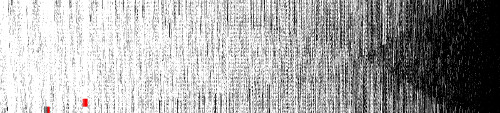
\includegraphics[width=\linewidth]{diagrams/2011-09-uptimes-truncated.jpg}
	\caption{The uptime matrix for a subset of all Tor relays in September 2011.
		Every row in the image represents one consensus, and every column
		represents one relay.  As a result, every pixel denotes the uptime
		status of a given relay at a given hour.  Black pixels mean ``online,''
		white pixels mean ``offline.''  Red blocks denote possible Sybil groups,
		as identified by Algorithm~\ref{alg:uptime}.}
	\label{fig:uptime-matrix}
\end{figure}

Once the columns are sorted, we run our algorithm to determine the distance
between two subsequent uptime sequences.  If the distance is under our
threshold, we mark both uptime sequences as red, to highlight them in manual
analysis.

\subsubsection{Fingerprint analysis}
\label{sec:fingerprint-analysis}
The information a Tor client needs to connect to an onion service is stored in a
distributed hash table (DHT) that consists of a subset of all Tor
relays, the onion service directories (HSDirs).  A daily-changing set of six
HSDirs are responsible for a given onion service and are asked by Tor clients
for information about the onion service they want to connect to.  An HSDir
becomes responsible for an onion service when its fingerprint is close to the
descriptor ID that is derived from the onion service's public key, a time stamp,
and additional information.
% https://gitweb.torproject.org/torspec.git/tree/rend-spec.txt:231
% descriptor-id = H(permanent-id | H(time-period | descriptor-cookie | replica))
Note that the DHT and all its HSDirs is known, making it possible to calculate
which index in the ring will be used by an onion service at a future point in
time~\cite{Biryukov2013a}.  Attackers can exploit this knowledge by repeatedly
generating identity keys until their fingerprint is close to the onion service's
index, thus becoming its HSDir.

We detect relays that change their fingerprint frequently by maintaining a
lookup table that maps a relay's IP addresses to a list of all fingerprints we
have seen it use.  We order the lookup table by the relays that changed the
fingerprints the most, and output the results.

\subsubsection{Nearest-neighbor search}
\label{sec:nearest-neighbor}
We frequently found ourselves in situations where exitmap discovered a malicious
exit relay and we were trying to find similar, potentially associated relays.
This involved extensive manual work, which we soon started to automate.  We
needed an algorithm for nearest-neighbor search, i.e., given a ``seed'' relay,
what are its $n$ most similar neighbors?  We define similarity as
\emph{redundancy in relay configuration} because similar relays share their
configuration parameters file such as ports, IP addresses, exit policies, or
bandwidth.  As a result, our algorithm works by comparing relay configurations.

A naive implementation would compare the seed relay to all other relays in the
consensus, which scales linearly.  We can do better by using \emph{metric trees}
because they guarantee $\mathcal{O}(\textrm{log}\,n)$ lookup, at the cost of
building a tree first.  Metric trees are a type of data structure to index data
in metric spaces and they require a distance metric in the mathematical sense,
i.e., the following four conditions must be met for three points $x$, $y$, and
$z$:
\begin{enumerate}
	\item $d(x, y) \geq 0$
	\item $d(x, y) = 0$ iff $x = y$
	\item $d(x, y) = d(y, x)$
	\item $d(x, z) \leq d(x, y) + d(y, z)$
\end{enumerate}

We use the Levenshtein distance as distance metric.  It takes as input two
strings and determines the minimum amount of modifications---insert, delete, and
modify---that are necessary to turn string $s_{1}$ into $s_{2}$.  The
Levenshtein distance can handle strings of different length and satisfies the
triangle inequality (number four in the above enumeration), so we are free to
use it in a metric tree.

Metric trees are only a concept.  As concrete implementation, we use the vantage
point tree (vp-tree)~\cite{Yianilos1993a}.  It recursively divides the given
data into two partitions; one that is close to the seed point according to a
threshold, and one that is not.  The vp-tree must first be built for the given
data, and it is then ready to perform nearest neighbor searches.  In our
implementation, building a vp-tree for 6,235 relays takes approximately 15
seconds.\footnote{Again, measured on a single Intel Core i7 2.9 GHz CPU.}
Subsequent nearest-neighbor lookups finish almost instantly.

% TODO (23 Nov 2015, 11:04am): \mynote{Still need to compare this to naive $n^{2}$ search.}

\subsubsection{Meaningful and useful results}
Systems that employ complex and opaque analysis techniques frequently suffer
from what Sommer and Paxson call the \emph{semantic gap}~\cite[\S
III.C]{Sommer2010a}, i.e., a system's output is difficult to act upon as its
meaning is unclear.  Our tools automate the \emph{detection} of Sybils, but the
process of \emph{blocking} them involves human interaction, which is why we took
special care to address the semantic gap.

We avoid the use of opaque classification methods as their output (frequently
distances in high-dimensional vector space) is difficult to interpret.  Instead,
we use the Levenshtein distance because its output is easy to understand and
retrace.  Figure~\ref{fig:visualization} further illustrates a visualization
that we developed for exploratory analysis, which is meant to complement
automated analysis.  The graph shows the similarities (edges) between four Tor
relays (vertices).

\begin{figure}[t]
	\centering
	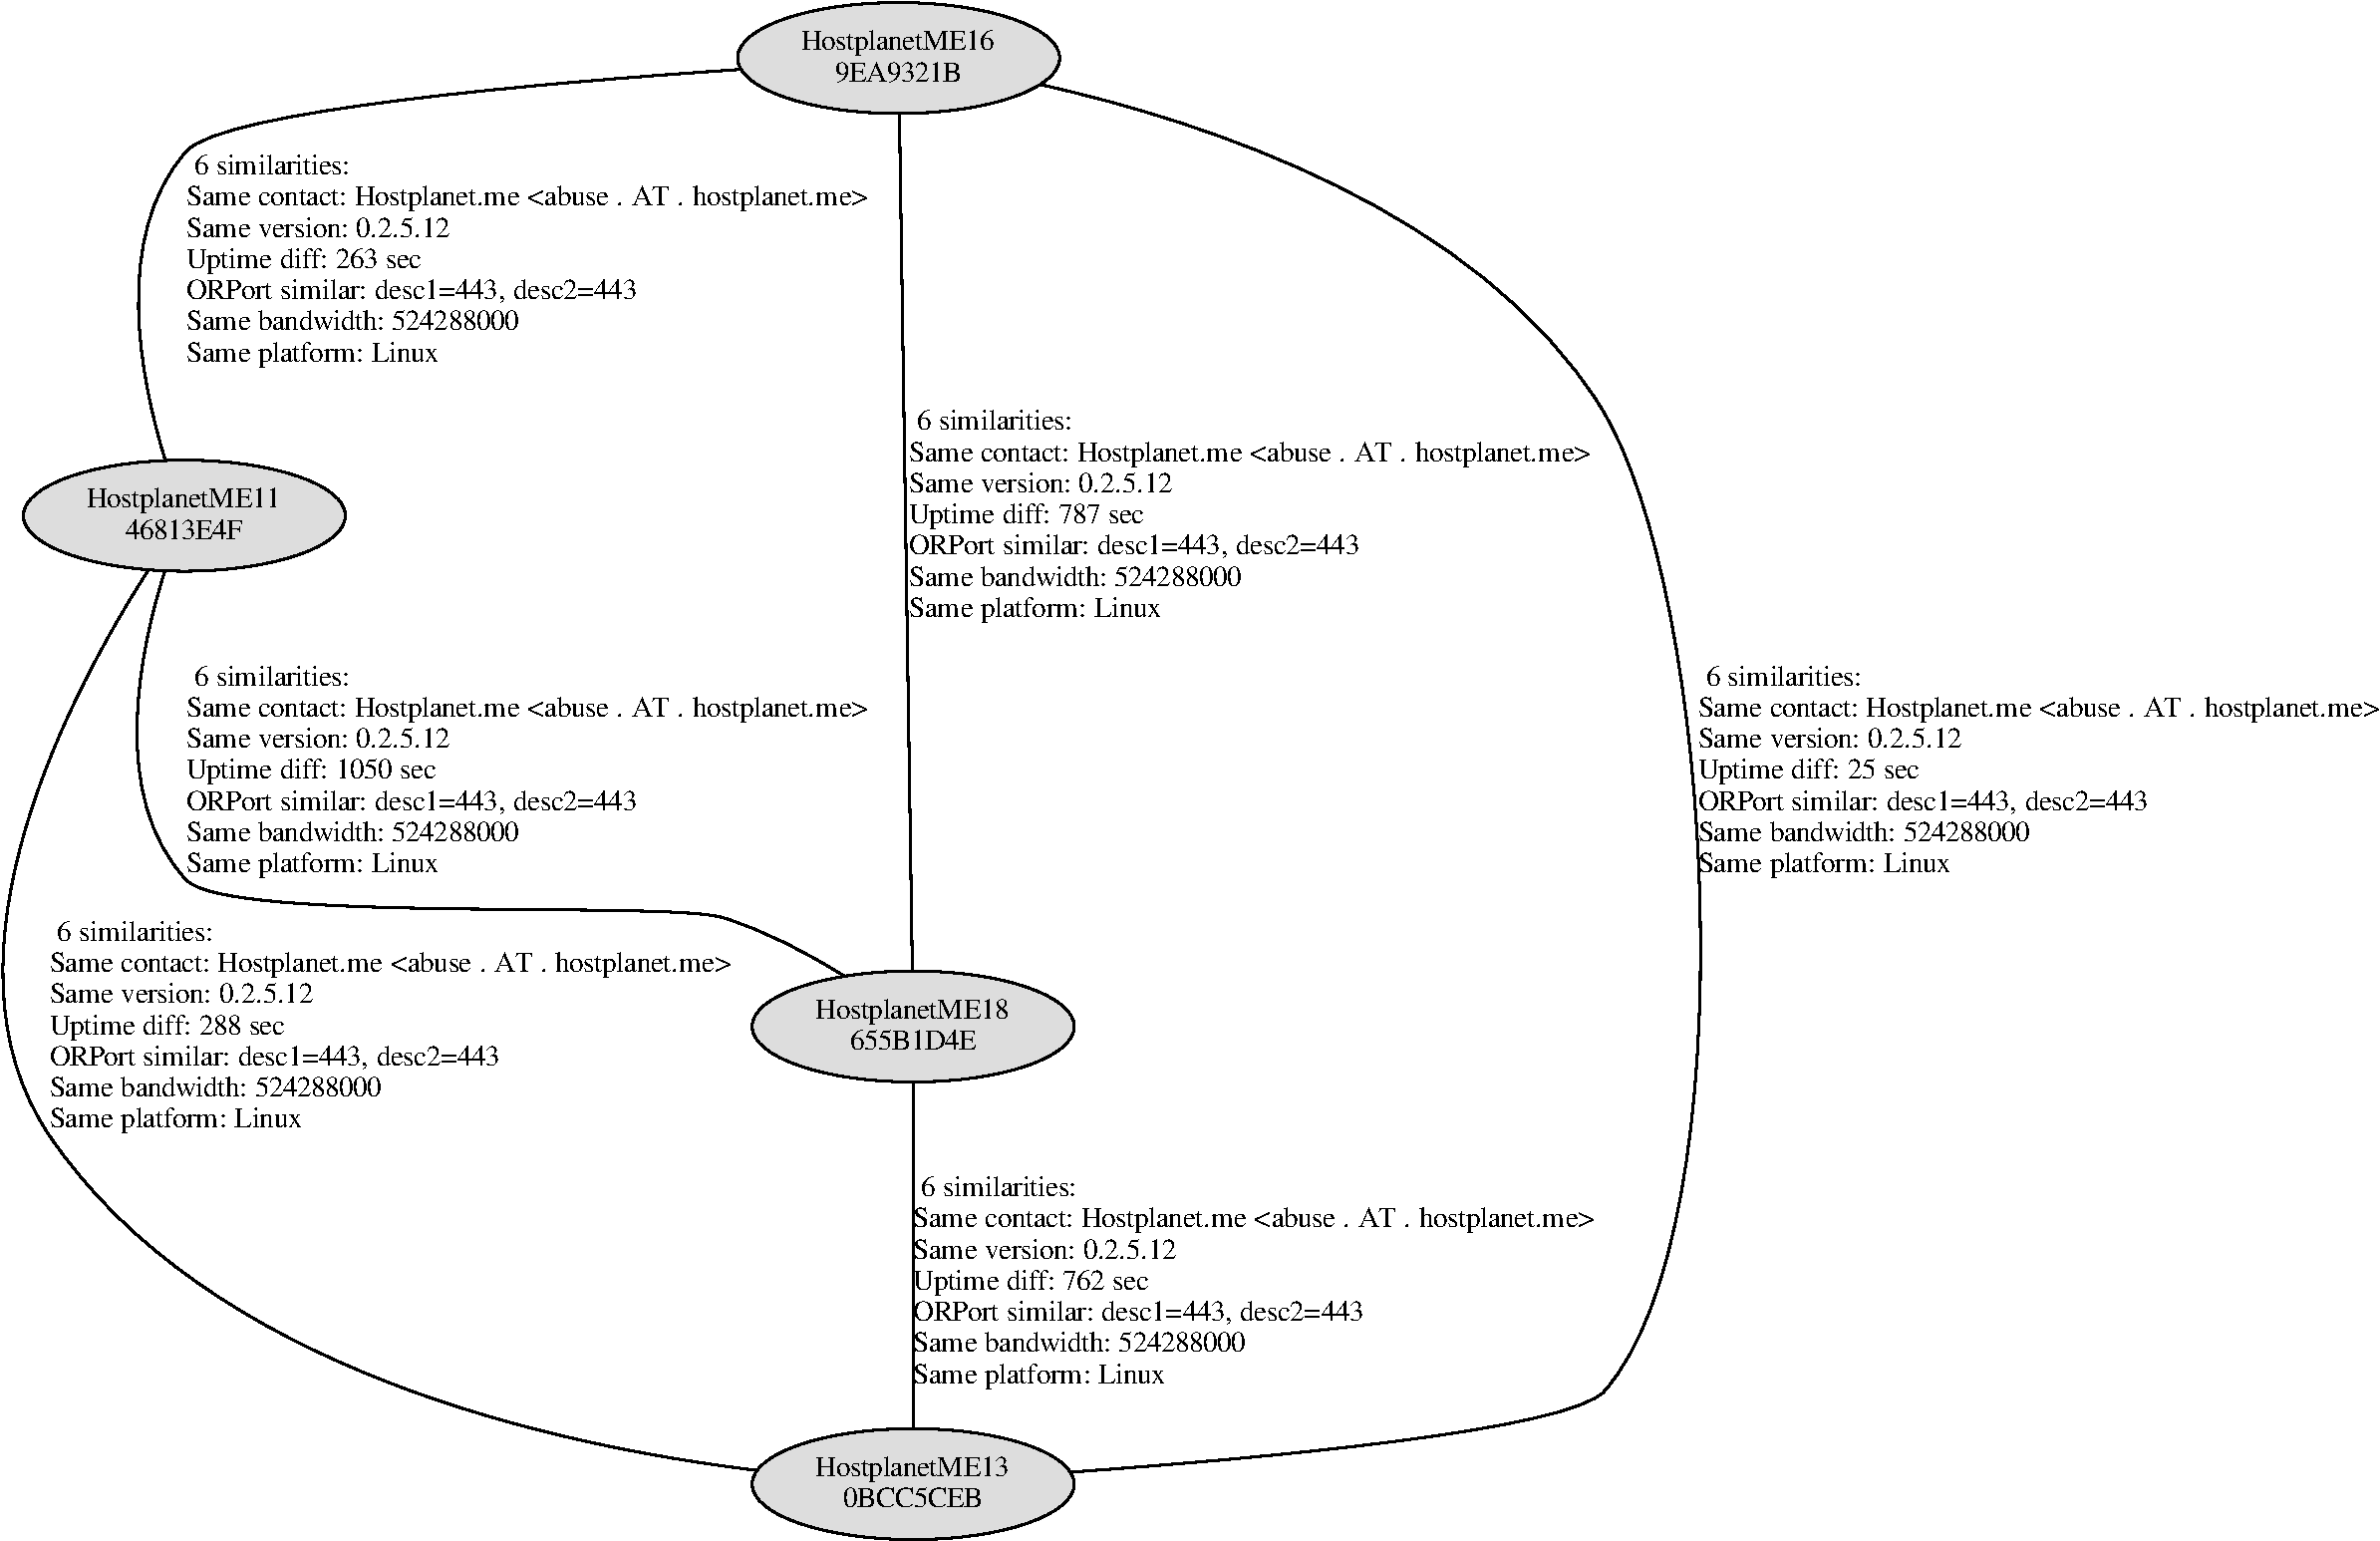
\includegraphics[width=\linewidth]{diagrams/visualization.pdf}
    \caption{Visualization of a Sybil cluster.  Vertices represent Tor relays
    and edges show the similarities between them.}
	\label{fig:visualization}
\end{figure}

We further reduce manual work by producing output that directory authority
operators can readily use to block Sybils, by simply pasting it into their
configuration files, for example:

{\footnotesize
\begin{verbatim}
# Reported-by: sybilhunter
# Date: Tue, 17 Nov 2015 10:07:27 -0000
# Reason: Sybil group that runs HTTPS MitM attacks.
# Fingerprints: B9D8842C3F0882BD7DE3BC81E6D8AEB5900C237D
#               83F2EEA05441D2BFA08BBDDD16AC19F79F162E42
#               A13BDD3858E0EBFB99F5F2D4C8866B69232CB5C2
AuthDirInvalid 12.34.56.78
AuthDirInvalid 1.23.4.56
AuthDirInvalid 123.4.56.7
\end{verbatim}
}

\noindent Finally, corresponding to the Unix tool design
philosophy~\cite{Pike1983a}, sybilhunter can produce CSV-formatted text output
that is easy to pipe into command line tools for further analysis using tools
such as cut, grep, and awk.

\subsection{Blocking Sybils}
\label{sec:blocking-sybils}
Once we discovered a seemingly harmful Sybil group, we reported it to The Tor
Project.  There are currently two ways for directory authorities to remove
relays, controlled by the options \texttt{AuthDirReject} and
\texttt{AuthDirInvalid}.  The former removes a relay from the consensus and the
latter takes away a relay's \texttt{Valid} flag.  While the relay is still
listed in the consensus, clients will not consider it for their first or last
hop in a circuit.

The majority of directory authorities, i.e., five out of eight, must agree on
either \texttt{AuthDirReject} or \texttt{AuthDirInvalid} to be set for a relay.
Only then will the block become active.  This mechanism is meant to distribute
the power of removing relays into the hands of a diverse set of people.
